
% this file is called up by thesis.tex
% content in this file will be fed into the main document

%: ----------------------- introduction file header -----------------------
% \begin{savequote}[90mm]
% Al parecer de acuerdo a los antecedentes, es razonablemente cierto que si existe cualquier movimiento relativo entre la Tierra y el Éter luminoso, éste tiene que ser lo suficientemente pequeño como para refutar completamente la explicación de la aberración de Fresnel.
% \qauthor{Albert Abraham Michelson}
% \end{savequote}


\chapter{Descripción de los polinomios de Zernike}
\label{cha:AppendixC}

% the code below specifies where the figures are stored
% \ifpdf
%     \graphicspath{{Anexo3/figures/PNG/}{Anexo3/figures/PDF/}{Anexo3/figures/}}
% \else
%     \graphicspath{{Anexo3/figures/EPS/}{Anexo3/figures/}}
% \fi
\graphicspath{{Figures/ApendiceC/}{../Figures/ApendiceC/}}
%-----------------Descripción_Polinomios_de_Zernike-------------

Éste apéndice ha sido tomado (previa autorización) de la tesis doctoral del profesor René
Restrepo Goméz. En él se espera dar a conocer los polinomios de
Zernike y mostrar cómo se puede llevar a cabo la composición de aberraciones ópticas en la base
de Zernike. Además se expone una tabla con la notación de los índices
de los polinomios usados en la implementación de nuestro método
de PD.   

Las aberraciones ópticas, conocidas como la diferencia entre la superficie del frente de onda teórico y la superficie del frente de onda real, pueden ser descritas a partir de una serie polinomial cualquiera, la más común son los llamados polinomios de Zernike \footnote[3]{Los polinomios de Zernike fueron desarrollados por el holandés Fritz Zernike a quien le fue otorgado el premio Nobel de Física en 1953.} \citepApC{Mahajan2011_ape3, schmidt2010_ape3}. Éstos son utilizados para reconstruir los mapas de frente de onda. Los polinomios de Zernike se  definen a partir de la Eq. \ref{eq:Ape3_1}  y la Eq. \ref{eq:Ape3_2},

%-----------Eq_1-------------
\begin{equation}\label{eq:Ape3_1}
 Z_{n}^{m}(\rho,\theta) = \sqrt[]{2(n+1)} R_{n}^{m}(\rho)G^{m}(\theta),
\end{equation}

%-----------Eq_2-------------
\begin{equation}\label{eq:Ape3_2}
 Z_{j}(\rho,\theta)= \left \{ \begin{matrix} \sqrt[]{2(n+1)} R_{n}^{m}(\rho)G^{m}(\theta) & m \neq 0
\\ R_{n}^{0}(\rho) & m = 0 \end{matrix}\right. 
\end{equation}

donde $n$ y $m$ denotan la variación radial y la frecuencia azimutal respectivamente. El índice $j$ se calcula con las variables $m$ y $n$ a partir de la Eq. \ref{eq:Ape3_3},

%-----------Eq_3-------------
\begin{equation}\label{eq:Ape3_3}
 j=\frac{n^{2}+2n+m}{2}.
\end{equation}

Y, las funciónes radial y azimutal están definidas como puede observarse en la Eq. \ref{eq:Ape3_4} y la Eq. \ref{eq:Ape3_5}, respectivamente,
 
%-----------Eq_4-------------
\begin{equation}\label{eq:Ape3_4}
 R_{n}^{m} (\rho)= \sum_{k=0}^{\frac{n-m}{2}} \frac{(-1)^{k}(n-k)!r^{n-2k}}{k!((\frac{n+m}{2})-k)!((\frac{m-n}{2})-k)!},
\end{equation}

%-----------Eq_5-------------
\begin{equation}\label{eq:Ape3_5}
 G^{m}(\theta)= \left \{ \begin{matrix} sen(m\theta) & \mbox{ si } j \mbox{ es par}
\\ cos(m\theta) & \mbox{ si } j \mbox{ es impar} \end{matrix}\right. 
\end{equation}

Por último, debe cumplirse la relación de la Eq. \ref{eq:Ape3_6}, es decir, los polinomios están normalizados sobre el círculo unitario,

%-----------Eq_6-------------
\begin{equation}\label{eq:Ape3_6}
 |Z_{j}(\rho,\theta)| \leq 1.
\end{equation}

La razón por la cual se puede describir cualquier frente de onda en términos de la Eq. \ref{eq:Ape3_1}, se debe a que dichos polinomios son linelamente independientes entre sí, dado que resultan del producto de dos funciones, una de las cuales varía en función del radio de una circunferencia unitaria, mientras que la otra varía en función del meridiano de la misma, y en consecuencia resultan ser ortogonales e independientes linealmente \citepApC{dai2008_ape3}. 

La Tabla \ref{Table1:Zernike}  muestra los primeros 36 polinomios de Zernike. Para la construcción de la tabla, se ha utilizado la convención de Noll \citepApC{Noll1976_ape3}. La fase puede ser parametrizada a través del frente de onda usando los polinomios de Zernike, y está descrita matemáticamente como en la Eq. \ref{eq:Ape3_7},

%-----------Eq_7-------------
\begin{equation}\label{eq:Ape3_7}
\phi(\rho, \theta)= 2\pi \sum_{j=1}^\infty a_{j}Z_{j}(\rho,\theta). 
\end{equation}

Una aberración típica parametrizada a través de los polinomios de Zernike es mostrada en la Fig. \ref{fig:aberracion}.

%-----------------Tabla_1-------------- 
\begin{table}[htbp]
\scalebox{0.9}{
\begin{tabular}{|c|c|c|c|c|}
\hline
\multicolumn{ 1}{|c|}{$\mathbf{Z_{j}}$} & \multicolumn{ 1}{c|}{\textbf{Nombre}} & \multicolumn{ 1}{c|}{$\mathbf{Z_{n}^{m}(\rho, \theta)}$} & \multicolumn{ 1}{c|}{\textbf{Índice n}} & \multicolumn{ 1}{c|}{\textbf{Índice m}} \\ \hline
$Z_{1}$ & piston & 1 & 0 & 0 \\ %\hline
$Z_{2}$ & x tilt  & $2\rho \cos \theta$ & 1 & 1 \\ %\hline
$Z_{3}$ & y tilt  & $2\rho \sin \theta$ & 1 & 1 \\ %\hline
$Z_{4}$ & defocus & $\sqrt{3}(2\rho^2-1)$ & 2 & 0 \\ %\hline
$Z_{5}$ & y primary astigmatism & $\sqrt{6}\rho^2 \sin (2\theta) $ & 2 & 2 \\ %\hline
$Z_{6}$ & x primary astigmatism & $\sqrt{6}\rho^2 \cos (2\theta) $ & 2 & 2 \\ %\hline
$Z_{7}$ & y primary coma & $\sqrt{8}(3\rho^3-2\rho) \sin \theta $ & 3 & 1 \\ %\hline
$Z_{8}$ & x primary coma & $\sqrt{8}(3\rho^3-2\rho) \cos \theta $ & 3 & 1 \\ %\hline
$Z_{9}$ & y trefoil & $\sqrt{8}\rho^3 \sin (3\theta) $  & 3 & 3 \\ %\hline
$Z_{10}$ & x trefoil & $\sqrt{8}\rho^3 \cos (3\theta) $ & 3 & 3 \\ %\hline
$Z_{11}$ & primary spherical & $\sqrt{5}(6\rho^4-6\rho^2+1) $  & 4 & 0 \\ %\hline
$Z_{12}$ & x secondary astigmatism & $\sqrt{10}(4\rho^4-3\rho^2)\cos(2\theta) $  & 4 & 2 \\ %\hline
$Z_{13}$ & y secondary astigmatism & $\sqrt{10}(4\rho^4-3\rho^2)\sin(2\theta) $ & 4 & 2 \\ %\hline
$Z_{14}$ & x tetrafoil & $\sqrt{10}\rho^4 \cos(4\theta) $ & 4 & 4 \\ %\hline
$Z_{15}$ & y tetrafoil & $\sqrt{10}\rho^4 \sin(4\theta) $  & 4 & 4 \\ %\hline
$Z_{16}$ & x secondary coma & $\sqrt{12}(10\rho^5-12\rho^3+3\rho) \cos \theta $ & 5 & 1 \\ %\hline
$Z_{17}$ & y secondary coma & $\sqrt{12}(10\rho^5-12\rho^3+3\rho) \sin \theta $ & 5 & 1 \\ %\hline
$Z_{18}$ & x secondary trefoil & $\sqrt{12}(5\rho^5-4\rho^3) \cos (3\theta) $ & 5 & 3 \\ %\hline
$Z_{19}$ & y secondary trefoil & $\sqrt{12}(5\rho^5-4\rho^3) \sin (3\theta) $ & 5 & 3 \\ %\hline
$Z_{20}$ & x pentafoil & $\sqrt{12}\rho^5 \cos (5\theta) $ & 5 & 5 \\ %\hline
$Z_{21}$ & y pentafoil & $\sqrt{12}\rho^5 \sin (5\theta) $  & 5 & 5 \\ %\hline
$Z_{22}$ & secondary spherical & $\sqrt{7}(20\rho^6-30\rho^4+12\rho^2-1) $  & 6 & 0 \\ %\hline
$Z_{23}$ & y tertiary astigmatism & $\sqrt{14}(15\rho^6-20\rho^4+6\rho^2)\sin (2\theta) $ & 6 & 2 \\ %\hline
$Z_{24}$ & x tertiary astigmatism & $\sqrt{14}(15\rho^6-20\rho^4+6\rho^2)\cos (2\theta) $ & 6 & 2 \\ %\hline
$Z_{25}$ & y secondary tetrafoil & $\sqrt{14}(6\rho^6-5\rho^4)\sin (4\theta) $ & 6 & 4 \\ %\hline
$Z_{26}$ & x secondary tetrafoil & $\sqrt{14}(6\rho^6-5\rho^4)\cos (4\theta) $ & 6 & 4 \\ %\hline
$Z_{27}$ &  & $\sqrt{14}\rho^6 \sin (6\theta) $  & 6 & 6 \\ %\hline
$Z_{28}$ &  & $\sqrt{14}\rho^6 \cos (6\theta) $ & 6 & 6 \\ %\hline
$Z_{29}$ & y tertiary coma & $4 (35\rho^7-60\rho^5+30\rho^3-4\rho)\sin \theta $ & 7 & 1 \\ %\hline
$Z_{30}$ & x tertiary coma & $4 (35\rho^7-60\rho^5+30\rho^3-4\rho)\cos \theta $ & 7 & 1 \\ %\hline
$Z_{31}$ &  & $4 (21\rho^7-30\rho^5+10\rho^3)\sin (3\theta) $ & 7 & 3 \\ %\hline
$Z_{32}$ &  & $4 (21\rho^7-30\rho^5+10\rho^3)\cos (3\theta) $  & 7 & 3 \\ %\hline
$Z_{33}$ &  & $4 (7\rho^7-6\rho^5)\sin (5\theta) $ & 7 & 5 \\ %\hline
$Z_{34}$ &  & $4 (7\rho^7-6\rho^5)\cos (5\theta) $ & 7 & 5 \\ %\hline
$Z_{35}$ &  & $4\rho^7 \sin (7\theta) $ & 7 & 7 \\ %\hline
$Z_{36}$ &  & $4\rho^7 \cos (7\theta) $ & 7 & 7 \\ %\hline
$Z_{37}$ & tertiary spherical & $3 (70\rho^8-140\rho^6+90\rho^4-20\rho^2 +1)$ & 8 & 0 \\ \hline
\end{tabular}
}
\caption{Los primeros 36 polinomios de Zernike}\label{Table1:Zernike}
\end{table}


%-----------------Figura_1--------------
\begin{figure}[h!]
\centering
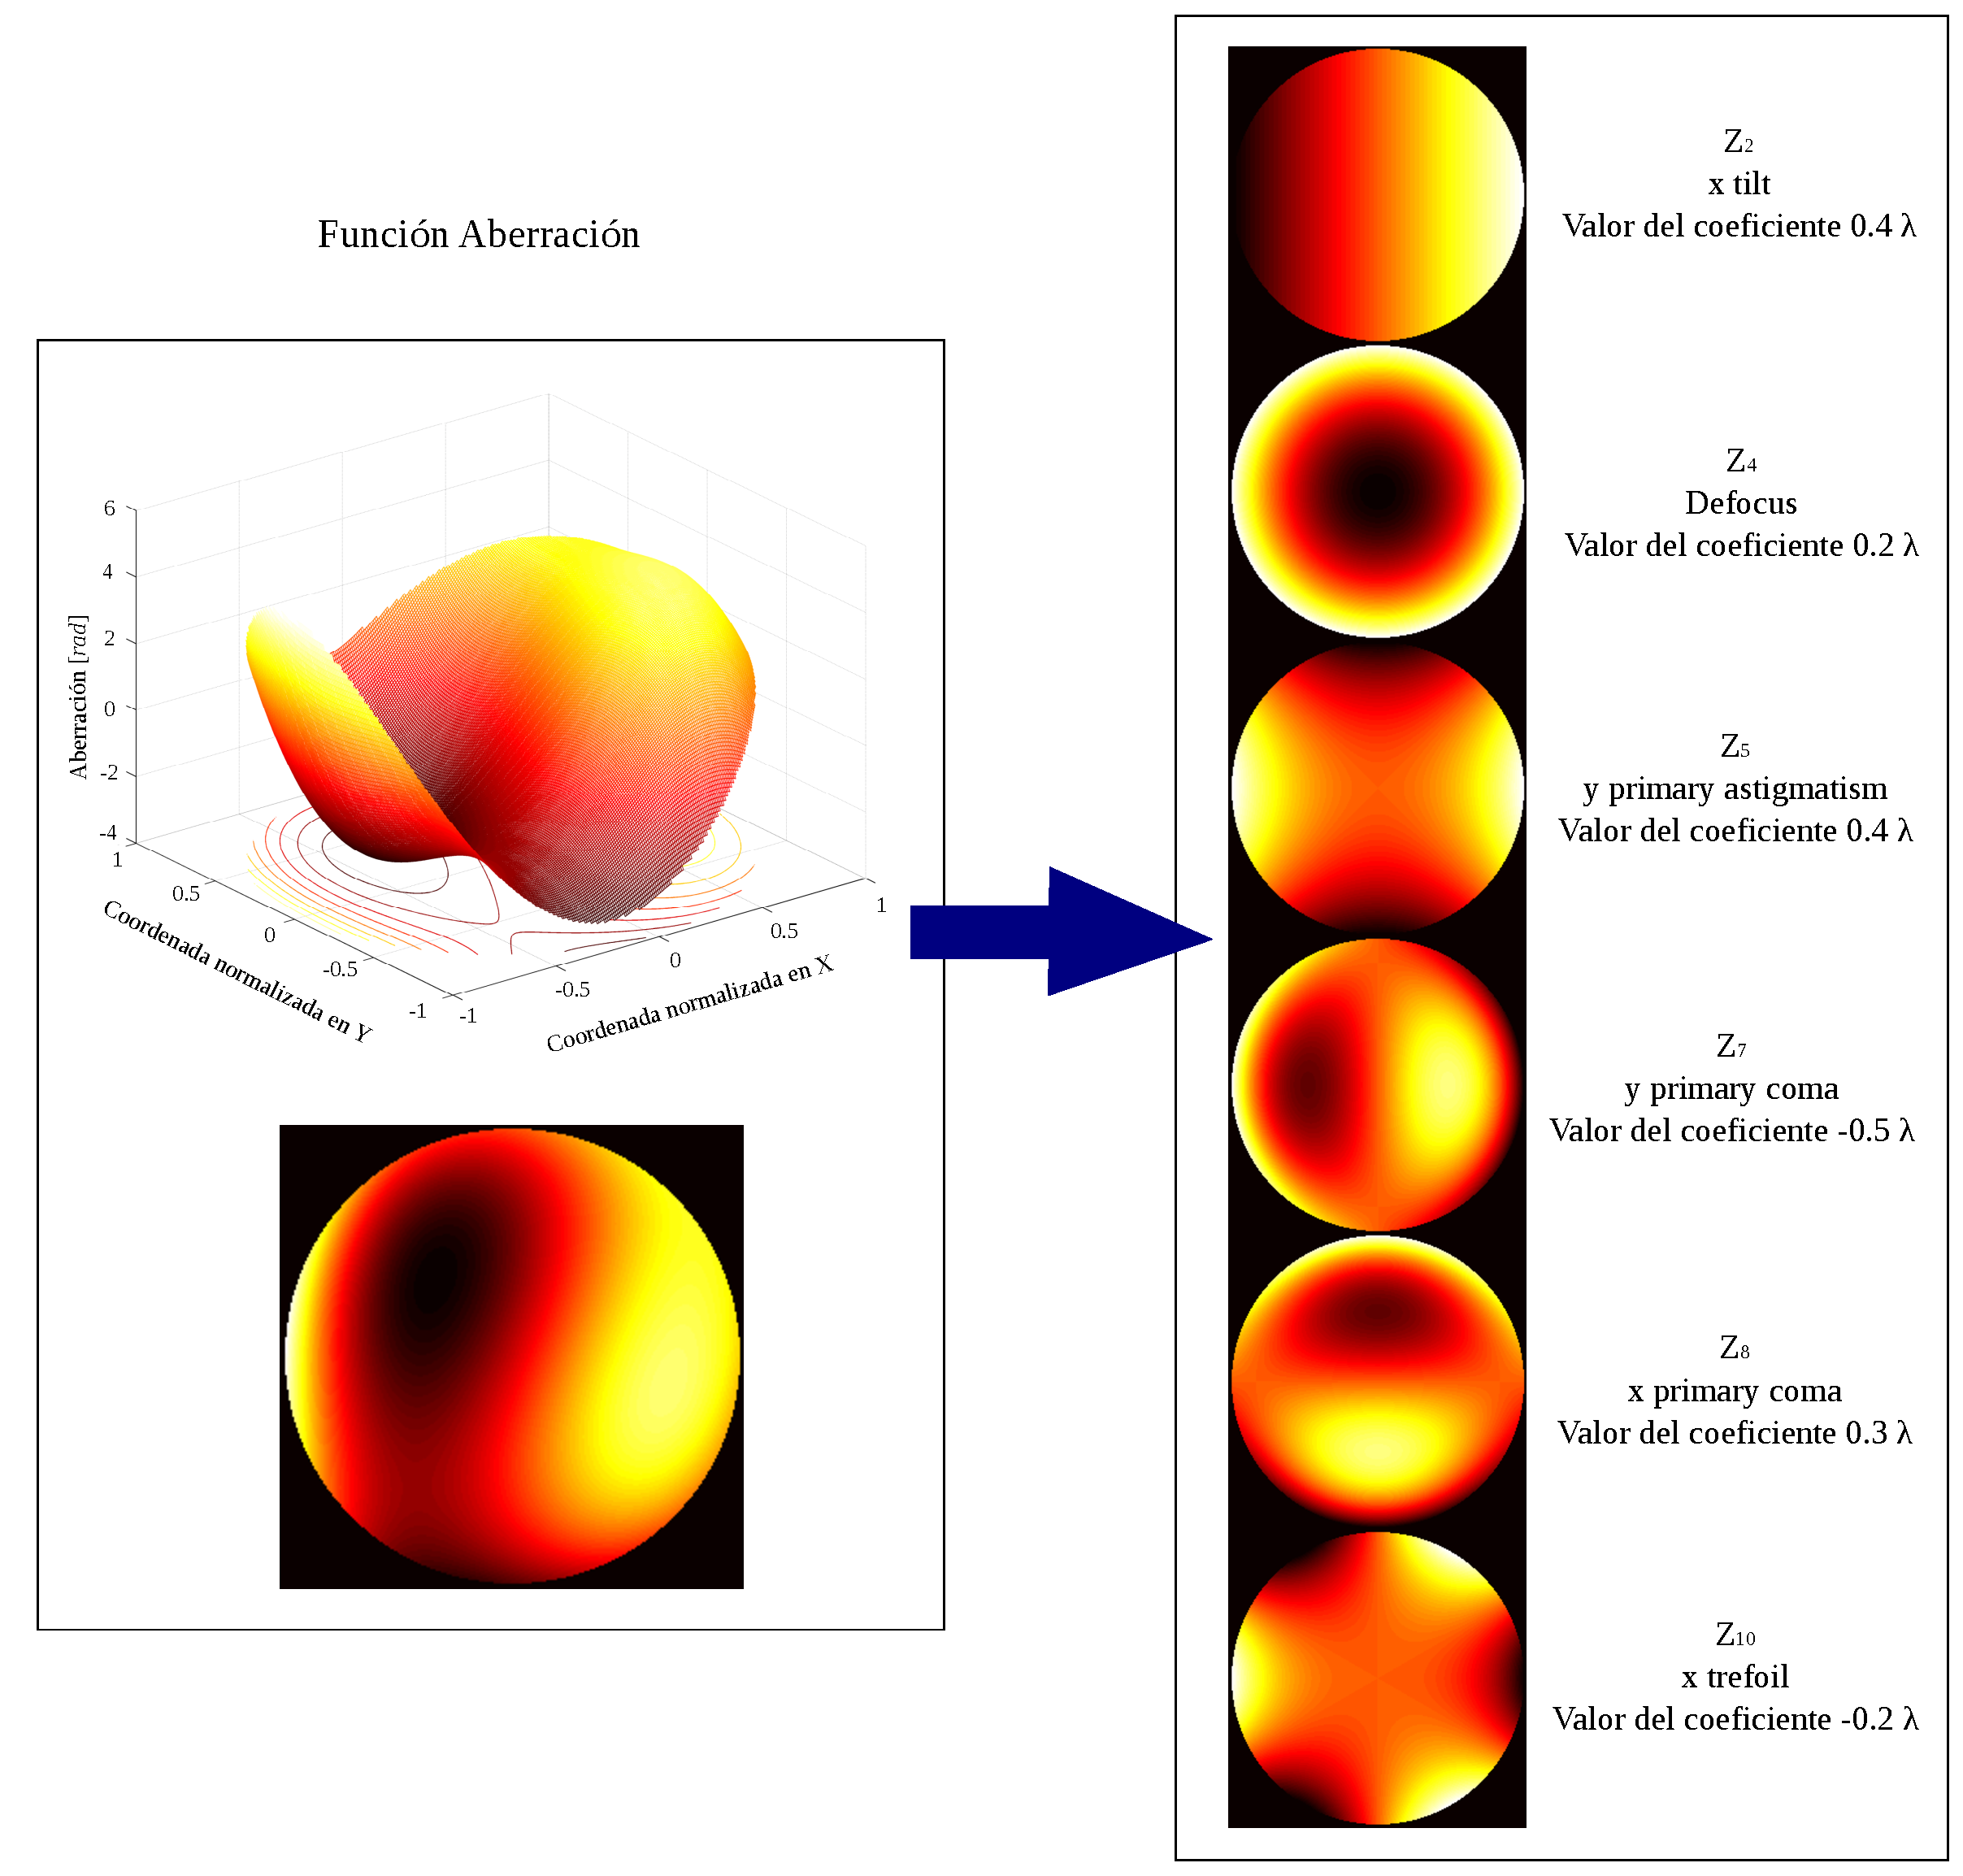
\includegraphics[width=14cm]{aberracion2.eps}\caption{\label{fig:aberracion} Ejemplo de una aberración del frente de onda parametrizada, a través de la suma de unos Polinomios de Zernike, cada uno con diferente peso.}
\end{figure}

%------------------------------------------------------------------------- 
\pagebreak
\bibliographystyleApC{ezspanish}
\bibliographyApC{References/ApeC}
